\documentclass[11pt,a4paper,twoside,openright]{report}

%frontespizio
\providecommand{\coursename}{Progetto di Ingegneria Informatica}
\providecommand{\annoacc}{2017-2018}
\providecommand{\principaladviser}{Prof. Andrea Bonarini}
\providecommand{\firstauthor}{İdil Su Erdenliğ}
\providecommand{\firstauthorid}{852772}
\title{Cognitive SLAM: Knowledge-Based Simultaneous Localization and Mapping}
\author{\firstauthor}

\usepackage{settings/frontesp}

\usepackage[italian]{hyperref}
\hypersetup{
    colorlinks,
    citecolor=black,
    filecolor=black,
    linkcolor=black,
    urlcolor=black
}
\newcommand{\autorefA}[1]{\hyperref[#1]{Algoritmo \ref{#1}}}

\usepackage{tabularx}
\usepackage{subfigure}
\usepackage{afterpage}
\usepackage{amsmath,amssymb}
\usepackage{amsthm}
\usepackage{settings/columnVectors}
\usepackage{rotating}  
\usepackage{fancyhdr}
\usepackage{algorithm}
\usepackage{algpseudocode}
\usepackage[epsilon]{backnaur}
\usepackage{tocbibind}
\usepackage[scriptsize]{caption} 
\usepackage{enumitem}
\usepackage{listings}
\usepackage{settings/languages}

\setlength{\oddsidemargin} {2. cm}
\setlength{\evensidemargin} {2. cm}
\addtolength{\oddsidemargin} {-0.4 cm}
\addtolength{\evensidemargin} {-0.4 cm}
\linespread{1.1}

\usepackage[italian]{babel}
\usepackage{lmodern}
\usepackage[utf8]{inputenc}
\renewcommand{\captionfont}{\normalfont \sffamily \itshape \small}

\setlength{\headheight}{15pt}
\pagestyle{empty}

\begin{document}
\pagenumbering{alph}
\titlep
\thispagestyle{empty} \normalfont \cleardoublepage
%\vspace{17cm}

%\large
\begin{flushright}
\itshape{A mio papà\dots}
\end{flushright}

\thispagestyle{empty}  \cleardoublepage
\pagenumbering{roman}
%\newpage
\chapter*{Sommario}

\addcontentsline{toc}{chapter}{Sommario}

Lo SLAM è uno dei principali problemi nello sviluppo di robot autonomi. Gli approcci correnti sono afflitti da un pesante costo computazionale e si comportano male in ambienti dinamici e disordinati; le performance di questi sistemi diventano ancora peggiori se si utilizzano sensori a basso costo, necessari per le applicazioni commerciali.
Questa tesi affronta il problema da un punto di vista nuovo e originale, usando feature ad alto livello come punti chiave e sfruttando la conoscenza di un esperto e un linguaggio fuzzy per riconoscerli, per tenere traccia di punti chiave forti e stabili e permettere mappe più intelligenti e una localizzazione robusta in ambienti complessi. L'idea fondamentale è quella di mantenere il tasso di errore della localizzazione limitato e ridurre il costo necessario a far navigare con successo un robot autonomo in un ambiente interno, usando solo i dati provenienti da una webcam e una unità di misura inerziale a basso costo.
Il principale problema è il riconoscimento di feature ad alto livello, come porte e scaffali, affrontato tramite un classificatore fuzzy ad albero, definito da un esperto, in modo da evitare fasi di allenamento e migliorare la generalità del riconoscimento.

\chapter*{Abstract}

\addcontentsline{toc}{chapter}{Abstract}

SLAM is one of the key issues in autonomous robots development. Current approaches are affected by heavy computational load and misbehave in cluttered and dynamic environment; their performance get even worse with low cost sensors, needed for market applications.
This thesis faces the problem in a new and original way, working with high level features as key points and using expert knowledge and a fuzzy language to detect them, in order to track strong and stable key points and allow smarter maps and robust localization in complex environments. The key idea is to keep the error rate of the localization process limited, and to reduce the cost of an autonomous robot to successfully navigate into an indoor environment using only the data from a webcam and a low cost Inertial measurement unit.
The main issue is the high level feature recognition, like doors and shelves, done by an expert-defined fuzzy tree classifier, in order to avoid training and improve generalization of recognition.
\thispagestyle{empty} \vspace*{.75truecm} \cleardoublepage
\tableofcontents
\listoffigures
\clearpage
%\chapter*{Ringraziamenti}

\addcontentsline{toc}{chapter}{Ringraziamenti}

Dopo cinque lunghi anni, sono finalmente giunto al momento di scrivere i ringraziamenti. Questo significa che sono sopravvissuto al ``Vietnam'' che è il Politecnico! Un'esperienza entusiasmante e tremendamente difficile.

Non voglio utilizzare questa pagina per fare i soliti ringraziamenti scontati: il professore mi ha aiutato, la famiglia mi ha sostenuto... Beh, penso che queste cose, seppure vere, non siano i motivi fondamentali per cui valga la pena di spendere delle parole.

Piuttosto, voglio ringraziare il Professor Bonarini per avermi dato una sfida difficile da affrontare, una sfida che mettesse alla prova le mie capacità fino al limite e che mi ha permesso di imparare così tante cose che, se me lo avessero detto prima, non ci avrei creduto. Lo ringrazio perchè devo a lui, e ai suoi collaboratori (come il buon Martino!), tutte le cose che ho imparato e che fanno la differenza tra uno studente qualunque e un vero ingegnere.

Voglio ringraziare anche Davide Cucci, per il suo fondamentale aiuto nella parte di localizzazione, quando ormai credevo di doverla escludere dalla tesi (E comunque il telefono non ha suonato!).

Voglio ringraziare anche Andrea Romanoni per essere riuscito a rispondere alle mie domande anche sotto l'ombrellone!

Voglio ringraziare i ``Nerd della prima fila'' per essere riusciti a:
\begin{itemize}[noitemsep, nolistsep]
 \item Farsi sgridare dal proprio relatore.
 \item Farsi bersagliare da gessi.
 \item Farsi sgridare da persone a caso per il casino in aula studio.
 \item Fare battute sconvenienti.
 \item Riprodurre musica e filmati sconvenienti (sempre nelle aule studio, ovvio!).
 \item Aprire siti sconvenienti da usare come esempi di applicazioni.
 \item Farsi prendere in giro perfino dai prof per la ``nerditudine''.
\end{itemize}

Voglio sottolineare che io non c'entro ASSOLUTAMENTE niente con tutte queste malefatte! Ok\dots forse 2\dots 3\dots volte\dots

Voglio infine ringraziare la mia famiglia per avermi sempre amato. Forse avrei potuto arrivare qui dove sono ora e essere quello che sono ora senza il supporto economico, gli sforzi per permetterci di seguire le lezioni e tutto il necessario ad affrontare una università impegnativa come il Politecnico. Ma sicuramente non sarei arrivato da nessuna parte senza il loro affetto. Perchè la cosa che più importa in una famiglia è sapere che la tua famiglia ci sarà sempre e comunque per te, qualsiasi cosa accada, proprio perchè si è una famiglia. Vi voglio bene.

Grazie.

\thispagestyle{empty} \vspace*{.75truecm} \normalfont \cleardoublepage
\pagestyle{plain}\renewcommand{\chaptermark}[1]{\markboth{\chaptername\ \thechapter.\ #1}{}} 
\renewcommand{\sectionmark}[1]{\markright{\thesection.\ #1}}         
\fancyhead[LE,RO]{\bfseries\thepage}    
                                        
\fancyhead[RE]{\bfseries\leftmark}    
\fancyhead[LO]{\bfseries\rightmark}     
\renewcommand{\headrulewidth}{0.3pt} 
\pagenumbering{arabic}
\thispagestyle{plain}

\include{chapters/Introduction}
\chapter{State of the Art}
\label{cap:statoArte}
\thispagestyle{empty}

\begin{quotation}
{\footnotesize
\noindent{\emph{Doc: Ecco perché non ha funzionato: c'è scritto ``Made in Japan''. \\
Marty: E che vuol dire Doc? Tutta la roba migliore è fatta in Giappone. \\
Doc: Incredibile!
} }
\begin{flushright}
Ritorno al Futuro, parte III
\end{flushright}
}
\end{quotation}
\vspace{0.5cm}

\section{Hierarchical Policy Search Algorithms}

$\mathcal{C},\mathcal{M}$

The high-dimensional, continuous state and action spaces is one of the main challenges in robot learning. Value function based methods require filling the complete action-state space with data
Tramite l'utilizzo di sonar, venivano estratte feature geometriche con cui veniva costruita la mappa, nella quale il robot si localizzava. 
Il problema principale della localizzazione è il ``problema della correlazione'': se la posizione della feature rispetto alla quale ci si localizza è affetta da incertezza, la conseguente stima della posizione effettuata rispetto a tale feature sarà affetta da un errore che dipende dall'errore della posizione della feature stessa. 
Questo problema diventa tanto più grave se si pensa che la posizione del robot in ogni istante non è nota a priori, ma deve essere stimata sulla base delle osservazioni precedenti. 

\`E necessario risolvere questo problema per evitare che l'errore della generazione della mappa e l'errore della stima della posizione divergano nel tempo. 
Per risolverlo, gli autori hanno spesso utilizzato un filtro di Kalman esteso.

Il filtro di Kalman è uno stimatore Bayesiano ricorsivo, che, supposto noto il modello lineare che regola la generazione dei dati e la loro osservazione, supposto che l'errore di misura e di modello siano gaussiani, restituisce la densità di probabilità del sistema osservato. 
Il filtro di Kalman, se utilizzato secondo le ipotesi, è uno stimatore ottimo dello stato del sistema osservato, secondo i minimi quadrati.
Tuttavia, nell'ambito della robotica, e in particolare nel problema della localizzazione, il modello di generazione e osservazione dei dati non può essere considerato lineare.
E' quindi necessario utilizzare un'estensione del filtro di Kalman al caso non lineare: il filtro di Kalman esteso (EKF) è una delle possibili soluzioni al problema. 
L'idea alla base del filtro di Kalman esteso è quella di lavorare sul modello linearizzato, stimato ricorsivamente dal modello non lineare sulla base della stima corrente.

Per avere una buona stima della posizione è necessario utilizzare un gran numero di feature, numero che cresce molto rapidamente con l'aumentare della dimensione dell'ambiente.
La complessità computazionale dell'approccio tradizionale basato sul filtro di Kalman esteso è $\mathcal{O}(N^3)$, con $N$ numero di feature, e quindi il tempo di calcolo diventa ben presto inaccettabile per prestazioni in tempo reale.
Per risolvere questo problema è stato introdotto in~\cite{Montemerlo02a} un nuovo algoritmo detto FastSLAM, che consiste nell'utilizzo del Particle Filter, e del filtro di Kalman esteso in combinazione. L'algoritmo associa ad ogni feature considerata, un filtro di Kalman esteso; la densità di probabilità congiunta, invece, viene calcolata sfruttando il Particle filter. 
Il Particle Filter è un altro stimatore Bayesiano ricorsivo, che, invece di un modello e dell'assunzione di rumore gaussiano, sfrutta metodi di tipo Monte Carlo per stimare la densità di probabilità del sistema che genera i dati.
Il risultato è un algoritmo che ha complessità computazionale $\mathcal{O}(N\log M)$, con $M$ numero di feature e $N$ il numero di particelle usate dal Particle Filter. 
Questo approccio rende il problema trattabile nella maggior parte dei casi, pur essendo pesante computazionalmente, dato che è necessario un elevato numero di particelle per avere una buona localizzazione.

Vista la particolarità del problema quando il sensore utilizzato è una videocamera monoculare, sono stati sviluppati algoritmi ad hoc.
Uno degli algoritmi più usati è PTAM~\cite{klein07parallel},~\cite{klein08improving}.
L'idea alla base di questo algoritmo è dividere in due thread separati il tracking e la creazione della mappa: un thread si occupa del tracking robusto di feature a basso livello, mentre l'altro thread si occupa della creazione della mappa. 
Per rendere efficiente il processo di mapping, solo i keyframe, ossia i frame che contengono maggiore informazione rispetto a quella già presente, vengono considerati.
Per rendere il processo di mapping robusto, vengono utilizzate tecniche batch per costruire la mappa, come ad esempio il bundle adjustment. Il bundle adjustment consiste in un processo iterativo di raffinamento della stima dei punti 3D ricostruiti e della posa della videocamera.
PTAM, tuttavia, nasce per applicazioni di realtà aumentata, e quindi necessita di una inizializzazione, per risolvere i problemi dell'acquisizione del primo keyframe e per gestire la scala della mappa.

Un approccio alternativo consiste nell'usare tutti i dati dell'immagine per eseguire la localizzazione, questo approccio è alla base, ad esempio, di DTAM, Dense Tracking and Mapping~\cite{conf/iccv/NewcombeLD11}. Questo algoritmo crea un modello denso dell'ambiente e usa l'allineamento della videocamera

Si sono dimostrati efficaci anche i metodi semi-diretti, come SVO~\cite{Forster2014ICRA}, Semi Direct Visual Odometry, un algoritmo che riesce a ottenere altissime prestazioni limitando l'estrazione delle feature ad alto livello ai soli keyframe, operando direttamente sulle intensità dei pixel nei frame successivi, eliminando le fasi computazionalmente più onerose, che sono l'estrazione e l'abbinamento delle feature. SVO si basa sulle idee di PTAM, ma ne migliora sia le prestazioni, riuscendo a essere computazionalmente più leggero, sia la precisione della mappa e della localizzazione riducendo di molto gli outlier.

Recentemente, stanno avendo molto successo i sistemi basati su sensori RGB-D~\cite{izadi2011kinectfusion},~\cite{henry2012rgb}. Questi sensori vengono utilizzati come scanner laser a basso costo per creare una mappa dell'ambiente. Tuttavia, sono soggetti a molte limitazioni, non essendo stati progettati per questo scopo, e soffrono tra l'altro di un raggio d'azione limitato. Nonostante queste limitazioni i sistemi riescono comunque a ottenere buone prestazioni in ambienti indoor~\cite{sturm2012benchmark}.

\section{Rappresentazione del Mondo}

Sono noti diversi modi per rappresentare un ambiente tridimensionale.
Il più semplice possibile è quello di usare delle nuvole di punti, direttamente estratte dai sensori. Un'altra rappresentazione comune è quella di filtrare le nuvole di punti ottenute tramite una griglia di voxel, come, ad esempio, in~\cite{30724}.
Metodi più avanzati permettono una rappresentazione geometrica dell'ambiente con un minor uso di memoria, come, ad esempio, le mappe di quota, in cui una mappa a due dimensioni è estesa con il calcolo del valore medio di altezza di ciascun punto 2D~\cite{herbert1989terrain}, le mappe di quota estese~\cite{pfaff2007efficient}, che tengono conto di possibili aperture attraversabili dai robot, oppure le mappe di quota multi livello~\cite{4058725}, che riescono a descrivere complesse geometrie multi livello.

Tra le mappe più promettenti esistono le mappe basate sugli octree, che permettono un'efficiente rappresentazione in memoria sia dello spazio occupato sia dello spazio libero, pur potendo descrivere geometrie complesse. Inoltre, questo tipo di rappresentazione permette di scalare facilmente la risoluzione della mappa, permettendo di utilizzare la stessa mappa per compiti che richiedono una precisione differente.
Un'efficiente implementazione di questo tipo di mappa può essere trovata in \cite{hornung13auro}.

Recentemente, si sta sviluppando l'idea di rappresentare il mondo ad alto livello, incorporando informazioni semantiche e geometriche che possano essere utilizzate non solo dagli algoritmi di navigazione, ma anche per svolgere compiti ad alto livello e ragionamenti. Una possibile soluzione al problema è l'approccio basato su Scene Graph~\cite{6630614}. Sono stati sviluppati anche linguaggi specifici di dominio (DSL) per poter interagire ad alto livello, ad esempio generando istanze di oggetti a partire da un modello generico, come ad esempio in \cite{blumenthal2014towards}.

\section{Riconoscimento di Oggetti}

La quasi totalità degli algoritmi di riconoscimento di oggetti nell'immagine è basata su tecniche di machine learning.
Una delle classi di algoritmi più usati sono quelli basati sulle Haar-like feature~\cite{710772}.
Queste feature sono calcolate in aree rettangolari, all'interno delle quali vengono sommati i valori dell'intensità dei pixel. Le somme sono in seguito usate per calcolare differenze tra aree di interesse, per poter riconoscere feature geometriche quali angoli, linee o bordi.
Un efficiente algoritmo per il riconoscimento di oggetti è descritto in~\cite{Viola01rapidobject} ed è stato ampliato in~\cite{Lienhart02anextended}, e consiste nell'utilizzare in cascata una serie di classificatori via via più restrittivi; ognuno dei classificatori di ogni stadio è costruito attraverso una tecnica di boosting, ossia sono formati da un insieme di classificatori deboli che creano un classificatore complessivo più restrittivo. I classificatori di base sono solitamente alberi di decisione. Il classificatore complessivo dà una risposta binaria; per riconoscere effettivamente l'oggetto deve essere applicato tramite una finestra mobile su tutta l'immagine. \\
Un algoritmo simile è descritto in~\cite{journals/ijista/AbramsonSG07}, dove, però, invece che feature Haar-like, vengono utilizzati direttamente un insieme di pixel selezionati nell'immagine.

Un'altra importante classe di algoritmi è basata sulle feature HOG (Histogram of Oriented Gradients)~\cite{1467360}.

Queste feature sono ricavate contando le occorrenze dell'orientamento dei gradienti in sotto-blocchi dell'immagine.
Su queste feature si basa l'algoritmo descritto in~\cite{lsvm-pami}. Questo algoritmo è in grado di definire un oggetto a partire dalle sue parti, e quindi è robusto anche a occlusioni parziali dell'oggetto. Tuttavia è computazionalmente molto più pesante dell'approccio basato su feature Haar-like.

Più recenti sono i metodi basati sul deep learning. Tra questi, i più promettenti nel riconoscimento di oggetti sono basati sulle reti neurali convoluzionali. La particolarità di queste reti è di essere basata su kernel di nodi collegati in maniera fissa, e ripetuti per coprire tutta l'immagine. La struttura rigida sfrutta la località dell'informazione nell'immagine, e permette un training più efficiente.
Un esempio di applicazione si può trovare in~\cite{NIPS2012_4824}.

Metodi recenti, sfruttano sensori RGB-D, come ad esempio Kinect, per riconoscere oggetti nella scena, come ad esempio in~\cite{lai2012detection}. La maggior parte delle tecniche usate sono un'estensione delle tecniche già descritte, spesso estendendo i descrittori delle feature grazie alle informazioni sulla profondità.

\section{Reasoning}

I sistemi di ragionamento sono stati alla base dell'Intelligenza Artificiale fin dalla nascita ed hanno trovato sbocco in diverse applicazioni tra cui i sistemi esperti, per lungo tempo una delle branche dell'intelligenza artificiale più attive~\cite{buchanan1984rule}~\cite{davis1977production}~\cite{joseph1994riley}.

Con la maturazione della tecnologia per lo sviluppo dei sistemi esperti, e l'avvento di Internet, l'attenzione della ricerca collegata ai sistemi di ragionamento formale si è spostata dai sistemi esperti al web semantico.
Il linguaggio più diffuso per i sistemi di inferenza è il linguaggio OWL 2~\cite{owl2-overview},~\cite{owl2-primer}, fortemente basato sulle logiche descrittive che permettono un buon compromesso tra espressività, e complessità computazionale e mantengono la logica utilizzata decidibile.

Fin dai primi sistemi esperti si è riconosciuta l'importanza del trattamento dell'incertezza in sistemi di ragionamento che avessero a che fare con il mondo reale~\cite{davis1977production}, ed in particolare si è avuta una larga diffusione in moltissimi settori della logica fuzzy~\cite{Zadeh1965338}, adottata anche nel nostro lavoro.

Un esempio di reasoning applicato al riconoscimento delle immagini può essere trovato in~\cite{DBLP:journals/ivc/MaillotT08}, in cui feature a basso livello vengono estratte da un meccanismo di machine learning, e utilizzate da un sistema di inferenza che sfrutta una ontologia per l'analisi ad alto livello dell'immagine. Un altro esempio di utilizzo di sistemi di inferenza nel riconoscimento di oggetti si può trovare in~\cite{DBLP:journals/corr/abs-1301-4991}, dove viene utilizzato il linguaggio OWL per specificare una base di conoscenza e riconoscere tramite la conoscenza di dominio gli oggetti nell'ambiente.



\cleardoublepage
% ---- Bibliography ----
\bibliographystyle{plain}
\pagenumbering{Roman}
\bibliography{altro/bibliografia}

\appendix

\pagestyle{fancy} 
\fancyfoot{}                                               
\renewcommand{\chaptermark}[1]{\markboth{\appendixname\ \thechapter.\ #1}{}} 
\renewcommand{\sectionmark}[1]{\markright{\thesection.\ #1}}         
\fancyhead[LE,RO]{\bfseries\thepage}    
                                        
\fancyhead[RE]{\bfseries\leftmark}    
\fancyhead[LO]{\bfseries\rightmark}     
\renewcommand{\headrulewidth}{0.3pt} 

%\chapter{Concetti Fondamentali}
\label{app:concetti}
\thispagestyle{empty}

\begin{quotation}
{\footnotesize
\noindent{\emph{Doc: Ovviamente il continuum temporale è stato interrotto creando questa nuova temporale sequenza di eventi risultanti in questa realtà alternativa. \\
Marty: Che lingua è Doc? \\
Doc: Ah si, si, si, si, si! Lascia che ti spieghi. Immagina, che questa linea rappresenti il tempo\dots}}
\begin{flushright}
Ritorno al Futuro, parte II
\end{flushright}
}
\end{quotation}
\vspace{0.5cm}

Si introducono in questo capitolo di seguito i concetti fondamentali alla comprensione della tesi.

\section{Logica Fuzzy}
La logica fuzzy è una logica multi valore che permette di esprimere non solo la verità o la falsità di una affermazione, ma anche un grado di verità, che può essere qualsiasi numero tra 0 (ossia l'affermazione è falsa) e 1 (ossia l'affermazione è vera). Questa propriet\`a fa della logica fuzzy uno strumento appropriato per modellare aspetti del mondo reale quando si sia in presenza di incertezza.

Tra l'altro, grazie a questa logica è anche possibile esprimere concetti che in una logica a due valori sarebbero paradossali.
Ad esempio, la frase ``sono un bugiardo'', che nella logica a due valori risulta paradossale, nella logica fuzzy può assumere valori consistenti.

\subsection{Insiemi Fuzzy}
La logica fuzzy è basata fortemente sul concetto di insieme fuzzy. Un insieme fuzzy è un insieme la cui funzione di appartenenza può avere valori nell'intervallo $[0, 1]$.
I fuzzy set sono quindi definiti da una funzione di appartenenza $f$ definita su un dominio $D$, avente come codominio l'intervallo $[0,  1]$.  Formalmente un fuzzy et è definito come:

\begin{equation*}
 f:D\rightarrow [0, 1]
\end{equation*}

Si definisce variabile linguistica $X$, definita sulla variabile di base $u$ una tupla così definita:
\begin{equation*}
(X, T(X), U, G, M)
\end{equation*}

dove:

\begin{description}
 \item [X] è il nome della variabile.
 \item [T(X)] è un insieme di termini, detti anche valori linguistici, che costituiscono il dominio di X.
 \item [U] è il dominio della variabile di base $u$.
 \item [G] è una regola sintattica per generare l'interpretazione di X per ogni valore di u.
 \item [M] è una regola semantica che associa a X il suo significato.
\end{description}


Data una variabile $x$, è possibile definire più fuzzy set rispetto al suo dominio. Si parla di frame of cognition quando valgono le seguenti condizioni:
\begin{enumerate}
 \item L'intero dominio della variabile è coperto da almeno un fuzzy set con valore di verità maggiore di zero.
 \item Tutti i fuzzy set sono unimodali.
 \item Tutti i fuzzy set sono normali.
\end{enumerate}

Inoltre si parla di partizione fuzzy, se la somma delle funzioni di appartenenza di ogni fuzzy set in ogni punto del dominio è uguale a 1.

La normale teoria degli insiemi è contenuta nella teoria degli insiemi fuzzy. Infatti, un intervallo è un insieme fuzzy, con valore di verità di tutti gli elementi pari a 1. Anche i singoli elementi possono essere trattati, tramite il fuzzy set singleton, che ha valore di verità 1 per un solo elemento del dominio, e 0 per tutti gli altri.

\subsection{Operazioni sui fuzzy set}

Sui fuzzy set sono definite le seguenti operazioni:
\begin{itemize}
 \item unione
 \item intersezione
 \item complemento
 \item aggregazione
\end{itemize}

\subsubsection{Complemento}

Dato un insieme fuzzy $A$, con funzione di appartenenza $\mu_A$ il complemento è definito come:

\begin{equation*}
 c(\mu_A(x)) = \mu_{\neg A}(x)
\end{equation*}

Il complemento di insiemi fuzzy deve rispettare i seguenti assiomi:
\begin{enumerate}
 \item $c(0)=1$, $c(1)=0$ (condizioni al contorno)
 \item $c$ è una funzione continua.
 \item $c$ è involutiva, ossia $c(c(a))=a\, \, \forall a \in [0, 1]$
\end{enumerate}

l'unica funzione che rispetta i seguenti assiomi è la funzione:

\begin{equation*}
 c(x) = 1 - x
\end{equation*}

\subsubsection{Intersezione}

Dati due insiemi fuzzy $A$ e $B$, con funzione di appartenenza $\mu_A$ e $\mu_B$ l'intersezione  è definita come:

\begin{equation*}
 i(\mu_A(x), \mu_B(x)) = \mu_{A\cap B}(x)
\end{equation*}

L'intersezione di insiemi fuzzy deve rispettare i seguenti assiomi:

\begin{enumerate}
 \item $i(a, 1)=a$ (condizioni al contorno)
 \item $d\geq b \implies  i(a,d)\geq i(a,b)$ (monotonicità)
 \item $i(b,a) = i(a,b)$ (commutatività)
 \item $i(i(a,b),d)=i(a,i(b,d))$ (associatività)
 \item $i$ è una funzione continua
 \item $a\geq i(a,a)$ (sub-idempotenza)
 \item $a_1<a_2 \wedge b_1<b_2\implies i(a_1,b_1)<i(a_2,b_2)$ (monotonicità stretta)
\end{enumerate}

Non esiste un'unica funzione che rispetta questi assiomi. Ogni funzione che rispetta questi assiomi viene detta T-norm.
Esempi di T-norm sono l'operatore minimo e il prodotto tra i valori di verità.

\subsubsection{Unione}

Dati due insiemi fuzzy $A$ e $B$, con funzione di appartenenza $\mu_A$ e $\mu_B$ l'unione è definita come:

\begin{equation*}
 u(\mu_A(x), \mu_B(x)) = \mu_{A\cup B}(x)
\end{equation*}

L'unione di insiemi fuzzy deve rispettare i seguenti assiomi:

\begin{enumerate}
 \item $u(a, 0)=a$ (condizioni al contorno)
 \item $b \leq d \implies u(a,b) \leq u(a,d)$ (monotonicità)
 \item $u(a,b) = u(b,a)$ (commutatività)
 \item $u(a,u(b,d)) = u(u(a,b),d)$ (associatività)
 \item $u$ è una funzione continua
 \item $u(a,a) \geq a$ (super-idempotenza)
 \item $a_1< a_2 \wedge b_1 < b_2 \implies u(a_1,b_1)<u(a_2,b_2)$ (monotonicità stretta)
\end{enumerate}

Non esiste un unica funzione che rispetta questi assiomi. Ogni funzione che rispetta questi assiomi viene detta T-conorm, o S-norm.
Esempi di S-norm sono l'operatore massimo e la somma probabilistica tra i valori di verità.
La somma probabilistica $p$ tra due variabili $a$  e $b$ è definita come:

\begin{equation*}
 p = a+b - a\cdot b 
\end{equation*}

\subsection{Aggregazione}

Dato un insieme di fuzzy set $(A_1, \dots, A_n)$, con funzione di appartenenza $(\mu_{A_1}, \dots, \mu_{A_n})$ l'insieme fuzzy aggregato $A$ è definito come:

\begin{equation*}
   \mu_A(x) = h(\mu_{A_1}(x), \dots, \mu_{A_n}(x))
\end{equation*}

L'aggregazione di fuzzy set deve rispettare i seguenti assiomi:

\begin{enumerate}
 \item $h(0, \dots, 0)=0, h(1, \dots, 1)=1 $ (condizioni al contorno)
 \item $a_i \leq b_i\, \forall i \implies h(a_1, a_n) \leq h(b_1, b_n)$ (monotonicità)
 \item $h$ è una funzione continua
 \item $h(a, \dots,a)=a$ (idempotenza)
 \item $h(a_1,\dots,a_n) = h(a_i, \dots, a_j)\, \forall i,\dots, j\in [1,n]$ (simmetria) %%
\end{enumerate}

Non esiste un unica funzione che rispetta questi assiomi. Un esempio di operatore di aggregazione valido è la media generalizzata:
\begin{equation*}
 h(a_1, \dots, a_n) = \dfrac{(a_1^\alpha + \dots + a_n^\alpha)^{1/\alpha}}{n}
\end{equation*}



\subsection{Regole Fuzzy}

Una regola di inferenza fuzzy può essere considerata come un modello, un mezzo per definire una funzione tra un ingresso e una uscita.

Le regole fuzzy che consideriamo sono composte nel seguente modo:
\begin{verbatim}
 IF <antecedente> THEN <consequente>
\end{verbatim}

Dove l'antecedente è una formula logica ben formata è il conseguente è una o più proposizioni legate dall'operatore and.

Una formula ben formata è definita come:

\begin{itemize}
 \item Una proposizione è una formula ben formata
 \item Se ``A'' è una formula ben formata, anche ``not A'' è una formula ben formata.
 \item Se ``A'' e ``B'' sono formule ben formate anche ``A and B'', ``A or B'' sono formule ben formate.
 \item null'altro è una formula ben formata.
\end{itemize}

Una proposizione è definita come un assegnamento di una etichetta a una variabile fuzzy, del tipo
\begin{verbatim}
 <VARIABLE> IS <LABEL>
\end{verbatim}

esistono due tipi di regole:
\begin{description}
 \item [Regole linguistiche] note anche come regole di Mamdami, dove il conseguente è la congiunzione di più clausole linguistiche. Queste regole possono essere considerate come una funzione che mappa una configurazione di input in ingresso a una interpretazione simbolica dell'output desiderato. 
 \item [Regole di modello] note anche come regole di Takagi-Sugeno-Kosko. In questo tipo di regole le proposizioni nel conseguente sono del tipo: \verb|<VARIABLE> IS f(...)|. Questo tipo di regole legano un modello alla variabile di uscita. La funzione \verb|f| può essere definita in qualunque modo, e prende in input le variabili di base delle variabili linguistiche presenti sul lato sinistro della regola.

\end{description}


Un insieme di regole fuzzy forma una knowledge base. Le regole della knowledge base possono avere diversi pesi, in modo da rendere più importanti alcune regole specifiche, oppure evitare la preponderanza delle regole lunghe rispetto a quelle corte.
L'inferenza sulla knowledge base viene fatta come segue: 

\begin{enumerate}
 \item Dato un insieme di fatti noti, ossia variabili linguistiche di cui si conosce il valore, vengono selezionate solo le regole il cui antecedente contiene solo le variabili note.
 \item Viene calcolato il valore di verità del lato sinistro delle regole
 \item Se specificato, il valore di verità viene combinato con il peso della regola.
 \item Viene aggregato l'output da regole diverse che calcolano la stessa etichetta.
 \item Viene defuzzificato, eventualmente, l'output simbolico calcolato, oppure viene compiuta una approssimazione linguistica, ossia viene calcolata l'etichetta in output che meglio approssima, decisa una metrica, l'output simbolico calcolato (che può contenere più etichette per la stessa variabile)
\end{enumerate}

Esistono vari tipi di defuzzificazione. L'operazione di defuzzificazione viene applicata all'insieme di insiemi fuzzy ricavati per ciascuna variabile linguistica. I metodi più noti sono:
\begin{itemize}
 \item Centro di massa
 \item Bisettrice
 \item Media dei massimi
 \item Minor massimo
 \item Maggior massimo
 \item Centro dell'area più alta
\end{itemize}

Il metodo più usato in assoluto è il centro di massa applicato a singleton.

\section{Geometria della telecamera}

Verrà descritta brevemente la geometria della telecamera.
Una telecamera è un dispositivo in grado di acquisire immagini del mondo. Essa è composta da una lente e un piano dell'immagine, in grado di acquisire l'immagine. Nel nostro modello consideriamo la lente come estremamente sottile, in modo da non considerare le distorsioni radiali e tangenziali dovute alla lente. La lente è necessaria in quanto essa è in grado di convogliare tutta la luce proveniente da un determinato punto dello spazio in un unico punto (oppure in un'area di punti) nel piano immagine.

Chiamiamo asse ottico l'asse perpendicolare al piano dell'immagine passante per il centro della lente. Si chiama Principal Point l'intersezione tra l'asse ottico e il piano dell'immagine.
Chiamiamo distanza focale la distanza tra la lente e il piano dell'immagine.

\subsection{Geometria proiettiva}

La relazione tra le coordinate della telecamera e le coordinate dei punti del mondo è una relazione non lineare.
Dato un punto nello spazio $P=(X,Y,Z)$, la sua proiezione nel piano dell'immagine $p=(x,y)$ avrà le seguenti coordinate:

\begin{equation*}
 \begin{aligned}
  x = f\cdot \dfrac{X}{Z} \\
  y = f\cdot \dfrac{Y}{Z}
 \end{aligned}
\end{equation*}

Con $f$ distanza focale della telecamera.

Per semplificare il problema, viene usato un altro sistema di coordinate in cui la relazione considerata è una relazione lineare.
Queste coordinate sono dette coordinate omogenee, e uno spazio che le utilizza viene detto spazio proiettivo.

Le coordinate omogenee sono delle coordinate che per esprimere uno spazio a $n$ dimensioni, utilizzano $n+1$ coordinate. Le coordinate spaziali sono definite a meno di un fattore moltiplicativo, ovvero $P = \alpha\cdot P$.
La quarta coordinata ha inoltre un significato particolare. Se è diversa zero il punto rappresenta un punto reale dello spazio euclideo, altrimenti rappresenta una direzione, detto anche punto all'infinito.


\subsubsection{Piano immagine}
Modelliamo l'immagine con uno spazio proiettivo a due dimensioni, $\mathcal{P}^2$.
Un punto $X$ del piano immagine è definito come:
\begin{equation*}
  X=\colvec{3}{x}{y}{w}
\end{equation*}

E' possibile anche definire una retta $l$ nel piano immagine sempre utilizzando il vettore tridimensionale:

\begin{equation*}
  l=\colvec{3}{a}{b}{c}
\end{equation*}

Un punto $X$ appartiene a una retta $l$ se:

\begin{equation*}
 X^T\cdot l = 0
\end{equation*}

Equivalentemente si può dire che una retta $l$ passa per un punto $X$ se:

\begin{equation*}
 l^T\cdot X = 0
\end{equation*}

l'equazione di una retta è quindi definita come:

\begin{equation*}
 a\cdot x + b \cdot y+ c \cdot w = 0
\end{equation*}

Anche la retta quindi è definita a meno di un coefficiente moltiplicativo.
La retta che contiene tutti i punti all'infinito è detta linea all'infinito $l_\infty$.

Nello spazio a due dimensioni è estremamente semplice calcolare la retta passante per due punti o il punto intersezione di due rette. Basta usare il prodotto vettoriale tra due elementi. Per calcolare la retta $l$ passante per due punti scriviamo:

\begin{equation*}
 l = P_1 \times P_2
\end{equation*}

Per calcolare il punto di intersezione $P$ tra due rette:

\begin{equation*}
 P = l_1 \times l_2
\end{equation*}


E' possibile esprimere anche coniche nel piano proiettivo. Una conica $C$ è definita come:

\begin{equation*}
 C = \begin{pmatrix} a & b & c \\ b & d & e \\ c & e & f \\ \end{pmatrix}
\end{equation*}

Si può notare che la matrice è simmetrica. Questo avviene senza perdita di generalità.
Un punto appartiene a una conica se:

\begin{equation*}
 X^T\cdot C \cdot X = 0
\end{equation*}

Anche le coniche sono definite a meno di un coefficiente moltiplicativo.

Infine è possibile esprimere coniche duali. Se le coniche sono insieme di punti, le coniche duali sono insieme di linee.
Si può dimostrare che la conica duale $C^*$ alla conica $C$ è:
\begin{equation*}
 C^*=C^{-1}
\end{equation*}

una retta appartiene alla conica duale se:

\begin{equation*}
 l^T\cdot C^* \cdot l = 0
\end{equation*}

Lo spazio proiettivo a 2 dimensioni ha due punti notevoli detti punti circolari. Tutte le possibili circonferenze si intersecano nei punti circolari, che sono due punti immaginari:

\begin{equation*}
 \begin{aligned}
  I=\colvec{3}{1}{i}{0} & & J=\colvec{3}{1}{-i}{0}
 \end{aligned}
\end{equation*}

I punti circolari appartengono a $l_\infty$.

Questi due punti possono essere espressi in maniera compatta dalla conica duale ai punti circolari, una conica degenere, che può essere calcolata come:

\begin{equation*}
 C^*_\infty = I\cdot J^T + J\cdot I^T =\begin{pmatrix} 1 & 0 & 0 \\ 0 & 1 & 0 \\ 0 & 0 & 0 \\ \end{pmatrix}
\end{equation*}


\subsubsection{Mondo reale}
Modelliamo il mondo reale con uno spazio proiettivo a 3 dimensioni, $\mathcal{P}^3$.

Un punto $X$ del mondo reale è definito come:
\begin{equation*}
  X=\colvec{4}{x}{y}{z}{w}
\end{equation*}

E' possibile anche definire piano $\pi$ nel mondo reale utilizzando il vettore quadridimensionale:

\begin{equation*}
  \pi=\colvec{4}{a}{b}{c}{d}
\end{equation*}

Un punto $X$ appartiene a una piano $\pi$ se:

\begin{equation*}
 X^T\cdot \pi = 0
\end{equation*}

Equivalentemente si può dire che un piano $\pi$ passa per un punto $X$ se:

\begin{equation*}
 \pi^T\cdot X = 0
\end{equation*}

l'equazione di un piano è quindi definita come:

\begin{equation*}
 a\cdot x + b \cdot y+ c \cdot z + d \cdot w = 0
\end{equation*}

Anche il piano quindi è definito a meno di un coefficiente moltiplicativo.
Il piano che contiene tutti i punti all'infinito e, conseguentemente, tutti le rette all'infinito di tutti i piani dello spazio, si chiama piano all'infinito $\pi_\infty$. 

E' possibile esprimere anche quadriche nel piano proiettivo. Una quadrica $Q$ è definita come:

\begin{equation*}
 Q = \begin{pmatrix} a & b & c & d \\ b & e & f & g \\ c & f & h & i \\ d & g & i & l \\ \end{pmatrix}
\end{equation*}

Si può notare che la matrice è simmetrica. Questo avviene senza perdita di generalità.
Un punto appartiene a una quadrica se:

\begin{equation*}
 X^T\cdot Q \cdot X = 0
\end{equation*}

Anche le quadriche sono definite a meno di un coefficiente moltiplicativo.

Infine è possibile esprimere quadriche duali. Se le quadriche sono insieme di punti, le quadriche duali sono insieme di piani.
Si può dimostrare che la quadrica duale $Q^*$ alla quadrica $Q$ è:
\begin{equation*}
 Q^*=Q^{-1}
\end{equation*}

Un piano appartiene alla quadrica duale se:

\begin{equation*}
 \pi^T\cdot C^* \cdot \pi = 0
\end{equation*}

Lo spazio proiettivo a 3 dimensioni ha una conica notevole, detta conica assoluta, $\Omega_\infty$. La conica assoluta è l'intersezione di tutte le possibili sfere nel mondo reale. La conica assoluta è formata dall'unione di tutti i possibili punti circolari calcolati lungo tutti i possibili piani dello spazio.
La conica assoluta è contenuta in $\pi_\infty$.

La conica assoluta può essere espressa in maniera sintetica con la quadrica duale assoluta $\Omega^*_\infty$:

\begin{equation*}
 \Omega^*_\infty = I\cdot J^T + J\cdot I^T =\begin{pmatrix} 1 & 0 & 0 & 0 \\ 0 & 1 & 0 & 0 \\ 0 & 0 & 1 & 0 \\ 0 & 0 & 0 & 0 \\ \end{pmatrix}
\end{equation*}

\subsection{Trasformazioni Proiettive}

Si chiama trasformazione proiettiva una qualsiasi trasformazione lineare di coordinate di uno spazio proiettivo. Una trasformazione proiettiva è detta anche omografia.
Generalmente una trasformazione proiettiva è una trasformazione non lineare rispetto allo spazio euclideo che rappresenta tutti i punti che non sono all'infinito.
Una trasformazione proiettiva di coordinate è data dalla formula:
\begin{equation*}
 x' = \mathcal{H}(x) = H\cdot x
\end{equation*}

Nello spazio $\mathcal{P}^2$ le trasformazioni proiettive sono descritte da matrici $3\times3$, mentre nello spazio $\mathcal{P}^3$ le trasformazioni proiettive sono descritte da matrici $4\times4$.

Ci sono alcuni sotto casi di trasformazione prospettica importanti e utili anche ai fini di questa tesi:

\begin{itemize}
 \item Rotazioni
 \item Traslazioni
 \item Isometrie
 \item Similitudini
 \item Affinità
\end{itemize}

Verranno discusse in seguito con i loro invarianti.
Tutte le trasformazioni sono definite a meno di un fattore di scala. L'ultimo elemento della matrice può quindi essere normalizzato a 1.

\subsubsection{Isometrie}

Le isometrie sono le trasformazioni prospettiche più semplici. Esse sono sostanzialmente rototraslazioni, e quindi contengono come casi particolari le rotazioni e le traslazioni pure. Gli invarianti delle isometrie sono le lunghezze, gli angoli, la forma e la dimensione, la posizione relativa tra gli oggetti. Hanno 3 gradi di libertà nel piano e 6 nello spazio.

Una isometria è descritta dalla matrice:

\begin{equation*}
  H_I = \begin{pmatrix}
   R & t \\
   \overline{0} & 1 \\
  \end{pmatrix}
\end{equation*}

$R$ è una matrice di rotazione, quindi è una matrice ortogonale, $3\times 3$ nello spazio e $2\times 2$ nel piano.
$t$ è un vettore di traslazione, $2\times 1$ nel piano e $3\times 1$ nello spazio.

\subsubsection{Similitudini}
Le similitudini sono trasformazioni prospettiche più generali delle isometrie. Hanno un grado di libertà in più rispetto alle isometrie, essendo la scala degli oggetti non fissata. Gli invarianti sono il rapporto tra le lunghezze, gli angoli, la forma degli oggetti.

\begin{equation*}
  H_S = \begin{pmatrix}
   sR & t \\
   \overline{0} & 1 \\
  \end{pmatrix}
\end{equation*}

Dove $s$ è il fattore di scala.

\subsubsection{Affinità}
Le affinità sono ancora più generali rispetto alle similitudini. Hanno 6 gradi di libertà nel piano e 12 nello spazio. Gli invarianti della trasformazione sono il parallelismo e il rapporto tra due segmenti paralleli.

\begin{equation*}
  H_A = \begin{pmatrix}
   A & t \\
   \overline{0} & 1 \\
  \end{pmatrix}
\end{equation*}

Dove $A$ è una matrice qualsiasi,  $3\times 3$ nello spazio e $2\times 2$ nel piano.

\subsection{Geometria della telecamera e calibrazione}

La telecamera è uno strumento che trasforma dei punti nello spazio a 3 dimensioni in punti sull'immagine a 2 dimensioni. La telecamera dunque attua una trasformazione proiettiva $P$ tra i due spazi.
L'equazione che mappa i punti tra i due spazi è la seguente:
\begin{equation*}
 \colvec{3}{x}{y}{w} = P\cdot\colvec{4}{X}{Y}{Z}{W}
\end{equation*}

la matrice $P$ dipende da due fattori: i parametri intrinseci della telecamera e i parametri estrinseci.
I primi dipendono dalla costruzione della fotocamera, e sono la distanza focale, la dimensione e la forma dei pixel, la posizione del principal point. I secondi sono la posa della telecamera rispetto al mondo, ovvero la rototraslazione della telecamera rispetto al mondo.  
Possiamo allora scrivere $P$ nel seguente modo:
\begin{equation*}
 P = K \cdot \left[
    \begin{array}{c|c}
      R & t
    \end{array} 
\right]
\end{equation*}

Dove la matrice $K$ è la matrice dei parametri intrinseci della telecamera, detta anche matrice di calibrazione, $R$ e $t$ sono, rispettivamente, la matrice di rotazione ($3\times3$) e traslazione ($3\times1$) della camera rispetto all'origine delle coordinate del mondo.

La matrice $K$ è definita nel seguente modo:

\begin{equation*}
 K = \begin{pmatrix} f_x & 0 & t_x \\ 0 & f_y & t_y \\ 0 & 0 & 1 \\ \end{pmatrix} 
\end{equation*}

Dove $f_x$ e $f_y$ sono la distanza focale espressa in pixel lungo l'asse $x$ e l'asse $y$ rispettivamente, $t_x$ e $t_y$ sono le coordinate del principal point nel piano dell'immagine. \\

La calibrazione della camera, e quindi il calcolo di $K$, si basa sulle proprietà dell'immagine della conica assoluta, $\omega$.
L'immagine della conica assoluta è la proiezione della conica assoluta sul piano dell'immagine. L'immagine della conica assoluta gode di una interessante proprietà: dipende solamente da $K$ e non dalla posa delle telecamera, è quindi invariante rispetto alle traslazioni e alle rotazioni. Detta $H$ la generica omografia che mappa la conica assoluta nella sua immagine, possiamo scrivere:

\begin{equation*}
 \begin{split}
  \omega &= H^{-T}\cdot\Omega_\infty\cdot H^{-1} = H^{-T}\cdot H^{-1} = \left( H\cdot H^T \right)^{-1} \\
         &= \left( K\cdot R\cdot \left( K\cdot R \right)\right)^{-1} =  \left( K\cdot R\cdot R^T \cdot K^T \right)^{-1} \\
         &= \left( K\cdot K^T \right)^{-1}
 \end{split}
\end{equation*}

Il problema della calibrazione si riduce quindi a trovare l'immagine della conica assoluta e calcolare $K$ decomponendo $\omega$ tramite la decomposizione di Cholesky.

Le camere reali soffrono di distorsioni ulteriori oltre a quelle prospettiche, che non sono descritte correttamente dalla geometria discussa. Queste sono la distorsione radiale e tangenziale, che sono espresse da dei coefficienti aggiuntivi, che servono per esprimere relazioni non lineari. Questi coefficienti non saranno descritti in quanto, sebbene fondamentali per analizzare l'immagine, non sono stati usati in questa tesi, e il modello utilizzato potrebbe variare tra telecamere differenti.

\section{Algoritmi di estrazione Feature}

Presentiamo qui i principali algoritmi usati da questa tesi.

\subsection{Canny Edge detector}
L'algoritmo di Canny è in grado di estrarre i bordi da una immagine in scala di grigi. L'immagine risultante è una immagine binaria che per ogni pixel indica o meno la presenza dei bordi. L'algoritmo si basa sulle seguenti fasi:
\begin{enumerate}
 \item Riduzione del rumore tramite un kernel gaussiano.
 \item Estrazione dei bordi tramite un operatore differenziale (ad esempio l'operatore di Sobel).
 \item Soppressione dei non massimi, ossia tutti i punti che non sono massimi globali, ovvero i punti in cui la derivata seconda del gradiente si annulla, vengono scartati.
 \item Sogliatura del gradiente con isteresi: date due soglie, se il punto ha gradiente maggiore della soglia alta viene accettato, se il punto è inferiore alla soglia bassa viene scartato, se il punto è compreso tra due soglie e adiacente a un punto accettato, viene accettato.
\end{enumerate}

Questo algoritmo necessita di tre parametri: la dimensione del kernel gaussiano e le due soglie per il gradiente.

\subsection{Trasformata di Hough}

La trasformata di Hough è un algoritmo in grado di estrarre linee da un immagine dei bordi.
La trasformata di Hough si basa sulla trasformazione da coordinate cartesiane a coordinate polari dell'equazione della retta, ossia l'equazione:

\begin{equation*}
 y=m\cdot x + q
\end{equation*}

Viene trasformata in:

\begin{equation*}
 \rho = x\cdot \cos(\theta) + y\cdot \sin(\theta)
\end{equation*}

Si può quindi descrivere le rette con i parametri $\rho$ e $\theta$ utilizzando un intervallo limitato di valori. Si procede dunque a discretizzare in celle lo spazio dei parametri con precisione diversa per  $\rho$ e $\theta$. Ogni punto vota tutte le celle che descrivono (approssimativamente) una retta passante su di esso. I picchi nello spazio delle celle sono le rette individuate.

Una versione più efficiente di questo algoritmo è la trasformata di Hough probabilistica, si veda l'\autorefA{alg:PPHT}.

\begin{algorithm}[ht]
\caption{Progressive Probabilistic Hough Transform}
\label{alg:PPHT}
\begin{algorithmic}[1] 
\While{image is not empty}
 \State{Select a random single pixel $P$}
 \State{Update accumulator with the votes of $P$}
 \State{$image \leftarrow image \ \lbrace P \rbrace$}
 \If{highest peak modified > threshold} 
  \State{Look along a corridor specified by the peak in the accumulator} 
  \State{Find the longest segment $l$ with gaps not exceeding a given threshold.}
  \State{Remove the pixels in the segment from input image}
  \State{“Unvote” from the accumulator all the pixels from the line that have previously voted.}
  \If{The line is longer than the minimum lenght}
    \State{$Lines \leftarrow Lines \cup l$}
  \EndIf
  \EndIf
\EndWhile
\Return Lines

\end{algorithmic}
\end{algorithm}

\subsection{DBSCAN}

DBSCAN è un algoritmo di clustering. Dato un insieme di dati e definita una misura di distanza, raggruppa i punti in un cluster basandosi sulla densità. Vengono quindi separate le aree in cui si trova una maggiore concentrazione di punti. I parametri dell'algoritmo sono il numero minimo di vicini perché il punto non sia considerato rumore, e la massima distanza tra due punti per considerarli vicini. Il funzionamento è descritto nell'\autorefA{alg:DBSCAN}.
         
\begin{algorithm}[ht]
\caption{DBSCAN}
\label{alg:DBSCAN}
\begin{algorithmic}[1] 
\Function{DBSCAN}{D, eps, MinPts}
  \State{$C \leftarrow 0$}
  \ForAll{$P \in D$}
    \State{$Visited \leftarrow Visited \cup P$}
    \State{$N \leftarrow$ \Call{regionQuery}{P, eps}}
    \If{cardinality of N < MinPts}
    \State{$Noise \leftarrow Noise \cup P$}
    \Else
      \State{$C \leftarrow C + 1$}
      \State{\Call{expandCluster}{P, N, C, eps, MinPts}}
    \EndIf
  \EndFor
  
\EndFunction

\Function{expandCluster}{P, N, C, eps, MinPts} 
  \State{$C \leftarrow C \cup P$}
  \ForAll{$P' \in N$}
    \If{$P' \not\in Visited$}
      \State{$Visited \leftarrow Visited \cup P'$}
      \State{$N' \leftarrow$ \Call{regionQuery}{P', eps}}
      \If{cardinality of N' >= MinPts}
	\State{$N \leftarrow N \cup N'$}
      \EndIf
    \EndIf
    \If{$\forall C\, P\not\in C$}
      \State{$C \leftarrow C \cup P'$}
    \EndIf
  \EndFor
\EndFunction

\Function{regionQuery}{P, eps}
  \Return{all points within P's eps-neighborhood (including P)}
\EndFunction
\end{algorithmic}
\end{algorithm}


%\chapter{Il manuale utente}
\label{app:manuale}
\thispagestyle{empty}

\begin{quotation}
{\footnotesize
\noindent{\emph{Marty: Come puoi vedere il fulmine ha fatto saltare il microchip di controllo dei tempo-circuiti. L'allegato diagramma sch .. sch.. \\
Doc: Schematizzato. \\
Marty: ..schematizzato, ti permetterà di costruire un'unità sostitutiva con le componenti del 1955, riportando così la macchina del tempo a un perfetto funzionamento.
}
}
\begin{flushright}
Ritorno al Futuro, parte II
\end{flushright}
}
\end{quotation}
\vspace{0.5cm}

\section{Installazione e compilazione}

Per compilare il sistema in maniera completa è necessaria una istallazione completa di \href{http://www.ros.org/}{ROS} \footnote{http://www.ros.org/}. Si veda la guida ufficiale di ROS per conoscere i dettagli dell'istallazione del sistema. \`E necessario utilizzare ROS Hydro Medusa o superiore.
Inoltre è necessario installare i generatori di parser \verb|Flex| e \verb|Bison|.
\`E possibile compilare la libreria che implementa l'algoritmo di reasoning anche al di fuori di ROS, utilizzando semplicemente \verb|CMake|. In tal caso si raccomanda di installare anche le librerie \verb|Boost|.

Una volta installate le dipendenze necessarie, è possibile compilare i sorgenti. Per farlo, basta creare un workspace di catkin, aggiungere i package nella cartella src, e lanciare catkin\_make. Le compilazione avverrà nell'ordine corretto, rispettando le dipendenze tra i package.
\`E necessario aggiungere il file setup.bash nella cartella \verb|devel/| del workspace come script da eseguire nel vostro file .bashrc; ad esempio, se il workspace  si chiama catkin\_ws, e si trova nella home, basterà aggiungere al file .bashrc la linea:
\begin{verbatim}
source ~/catkin_ws/devel/setup.bash
\end{verbatim}

Per lanciare i singoli nodi si può utilizzare il programma rosrun. Ricordarsi di aggiungere gli argomenti da linea di comando e i parametri privati necessari subito dopo il nome del package e del nodo che si vuole lanciare. 
I parametri privati vengono specificati aggiungendo un ``\_'' prima del nome del parametro; il cui valore viene assegnato con il token ``:=''.

Ad esempio per lanciare il nodo c\_fuzzy\_reasoner nel package c\_fuzzy si può utilizzare il comando:

\begin{verbatim}
rosrun c_fuzzy c_fuzzy_reasoner -c knowledgebase.kb classifier.fuzzy
\end{verbatim}

Una alternativa per lanciare tutti i nodi contemporaneamente è usare un launchfile. Launchfile di esempio sono presenti nel package c\_slam.

Per lanciare l'intero sistema si può utilizzare il comando:

\begin{verbatim}
roslaunch c_slam c_slam.launch
\end{verbatim}


\section{Parametri e argomenti}

Di seguito sono elencati e spiegati i parametri utilizzati dai nodi. si veda il \autoref{app:concetti} per informazioni riguardo agli algoritmi.

\subsection{c\_vision\_detector e c\_vision\_recognition}

Questi nodi hanno bisogno necessariamente di parametri privati, senza i quali il loro funzionamento non è garantito.

\subsubsection{Canny}

Questi parametri sono utilizzati dall'algoritmo Canny Edge detector.

\begin{description}
 \item [canny/alpha] rappresenta il valore della soglia bassa, in proporzione alla soglia alta.
 \item [canny/apertureSize] rappresenta la dimensione del kernel con il quale applicare l'operatore di Sobel. Deve essere necessariamente un intero dispari e maggiore o uguale a 3. 
\end{description}

\subsubsection{Hough}

Questi parametri sono utilizzati per l'algoritmo di riconoscimento delle linee, detto trasformata di Hough probabilistica.

\begin{description}
 \item [hough/rho] risoluzione della distanza dall'origine delle rette espressa in pixel.
 \item [hough/teta] risoluzione dell'inclinazione delle rette, espressa in gradi.
 \item [hough/threshold] threshold per filtrare le linee dal rumore.
 \item [hough/minLineLenght] minima lunghezza delle linee riconosciute, espressa in pixel.
 \item [hough/maxLineGap] massima distanza tra due punti appartenenti alla stessa linea, in pixel.
\end{description}

\subsubsection{Line filtering}

Questi parametri vengono utilizzati dall'algoritmo che distingue le linee orizzontali e verticali dal rumore.

\begin{description}
 \item [filter/maxDeltaHorizontal] massima inclinazione delle rette orizzontali rispetto alla linea dell'orizzonte, in gradi.
 \item [filter/maxDeltaVertical] massima inclinazione delle rette verticali rispetto alla linea perpendicolare all'orizzonte, in gradi.
\end{description}


\subsubsection{Clustering}

Questi parametri servono per tarare il riconoscimento dei cluster. Sono utilizzati dagli algoritmi FAST, per riconoscere i keypoints, e DBSCAN per estrarre da essi i cluster.

\begin{description}
 \item [cluster/threshold] threshold per l'estrazione di keypoints dall'immagine.
 \item [cluster/minPoints] numero minimo di punti necessari a definire un cluster.
 \item [cluster/maxDistance] massima distanza tra i punti di un cluster.
\end{description}

Questi parametri non sono necessari nel nodo c\_vision\_detector.

\subsubsection{Classifier}

Questi parametri sono utilizzati dai nodi di visione quando vengono preparate le richieste di reasoning, e quindi sono di fatto utilizzati nel classificatore fuzzy.

\begin{description}
 \item [classifier/threshold] threshold da utilizzare nella classificazione delle feature.
\end{description}

\subsection{c\_fuzzy\_reasoner}

Per lanciare il reasoner è necessario specificare dei parametri da linea di comando.

\begin{description}
 \item [-h] stampa il messaggio di aiuto 
 \item [-r knowledgebase] crea il servizio di reasoning basato sulla knowledgebase specificata.  
 \item [-c knowledgebase classifier] crea il servizio di classificazione a partire dalla knowledgebase e dal classificatore specificati. 

\end{description}


%\chapter{Esempio di impiego}
\label{app:esempio}
\thispagestyle{empty}

\begin{quotation}
{\footnotesize
\noindent{\emph{Doc: Scusa, la rozzezza di questo modello ma non ho avuto il tempo di farlo in scala e di dipingerlo. \\
Marty: Va bene, va bene.
} }
\begin{flushright}
Ritorno al Futuro, parte III
\end{flushright}
}
\end{quotation}
\vspace{0.5cm}

Mostriamo in questo capitolo il sistema hardware e software utilizzato per testare i concetti, gli algoritmi e le metodologie presentate in questa tesi.

\section{Robot}
Il robot preso in considerazione per i nostri test sperimentali è un quadrotor. Abbiamo utilizzato l'A.R. Drone, prodotto da Parrot. 
Il quadrotor utilizzato è dotato di una telecamera HD con risoluzione $640\times 480$, tuttavia nella tesi sono state utilizzate immagini a $320\times 240$, a 30 frame al secondo.
La qualità delle immagini è scadente, e sono affette da pesanti problemi di refresh.
Il robot possiede anche una unità di misura inerziale economica e un magnetometro.
Inoltre il robot possiede una telecamera inferiore, di risoluzione $320\times 240$, la cui qualità dell'immagine è molto peggiore rispetto alla telecamera frontale, che tuttavia non è stata sfruttata per lo svolgimento di questa tesi.

\'E stato scelto di utilizzare questo quadrotor per alcuni validi motivi:
\begin{itemize}
 \item L'hardware è a basso costo, e il quadrotor si trova in commercio a un prezzo relativamente basso.
 \item Il robot in questione ha 6 gradi di libertà nello spazio, questo rende possibile lo studio di un sistema di localizzazzione e mapping in 3 dimensioni.
 \item Il robot è già integrato con ROS.
\end{itemize}


\section{Hardware e software di controllo}
Per controllare il quadrotor e lanciare l'algoritmo di controllo è stato utilizzato un portatile dotato di processore Intel Core i7-4500U, e 4GB di RAM DDR3.
Il portatile utilizzato si occupava, oltre che di gestire l'algoritmo di controllo, di visualizzare output di debug.
Per il controllo del drone è stato utilizzato il driver \textit{ardrone\_autonomy}, disponibile nei repository di ROS.
Per muovere il quadrotor è stato utilizzato un joystick, integrato con ROS tramite il nodo \textit{joy}, anchesso presente nei repository ufficiali di ROS.
Per impartire comandi dal joystick al quadrotor ci si è avvalsi di un controllore già implementato nel package  \textit{ardrone\_tutorials}, che fornisce anche una finestra che mostra l'immagine presa direttamente dalla telecamera del drone.

\section{Classificatore utilizzato}

Il classificatore utilizzato prende in input rettangoli e cluster.
La struttura del classificatore è data dal seguente file:

\begin{lstlisting}[language=fuzzyClassifier]
CLASS Rectangle HIDDEN
	VARIABLES
		xMin;
		xMax;
		yMin;
		yMax;
		formFactor;
		area;
	END_VARIABLES
END_CLASS

CLASS Cluster HIDDEN
	VARIABLES
		x;
		y;
	END_VARIABLES
END_CLASS

CLASS WhiteBoard extends Rectangle
	area is Big;
	formFactor is Wide;
END_CLASS

CLASS LargeWhiteBoard extends Rectangle
	area is VeryBig;
	formFactor is VeryWide;
END_CLASS

CLASS Cabinet extends Rectangle
	area is Huge;
	formFactor is Medium;
END_CLASS

CLASS CabinetDoor extends Rectangle
	area is VeryBig;
	formFactor is Narrow;
END_CLASS

CLASS PossibleDoor extends Rectangle
	formFactor is VeryNarrow;
	area is VeryBig;
END_CLASS

CLASS Door extends PossibleDoor
	
	CONSTANTS
		height = High;
	END_CONSTANTS
	
	Handle.x is Lateral on(xMin, xMax);
	Handle.y is Centered on(yMin, yMax);

END_CLASS

CLASS Handle extends Cluster	
	x is Lateral on Door(xMin, xMax);
	y is Centered on Door(yMin, yMax);
END_CLASS
\end{lstlisting}

La knowledgebase di riferimento è definita nel modo seguente:

\begin{lstlisting}[language=fuzzyKnowledgebase]
FUZZIFY_CLASS Rectangle
	FUZZIFY formFactor
		VeryNarrow := tra(2600, 2700, 2900, 3000);
		Narrow := tra(1900, 2000, 2600, 2700);
		Medium := tra(900, 1000, 1100, 1500); 
		Wide := tra(850, 900, 920, 970);
		VeryWide := tra(700, 800, 850, 900);
	END_FUZZIFY
	
	FUZZIFY area
		Big := tor(7000, 7500);
		VeryBig := tor(9000, 10000);
		Huge := tor(20000, 25000);
	END_FUZZIFY
END_FUZZIFY_CLASS

FUZZIFY_CLASS Cabinet
END_FUZZIFY_CLASS

FUZZIFY_CLASS CabinetDoor
END_FUZZIFY_CLASS

FUZZIFY_CLASS WhiteBoard
END_FUZZIFY_CLASS

FUZZIFY_CLASS LargeWhiteBoard
END_FUZZIFY_CLASS

FUZZIFY_CLASS PossibleDoor
END_FUZZIFY_CLASS

FUZZIFY_CLASS Door

	FUZZIFY_PREDICATE ?x
		Lateral := (?x is Left) or (?x is Right);
		Centered := (?x is Centered);
		
		FUZZIFY ?x
			Left := tol(20, 30);
			Centered := tra(40, 50, 55, 60);
			Right := tor(70, 80);
		END_FUZZIFY
		
	END_FUZZIFY_PREDICATE	
	
END_FUZZIFY_CLASS

FUZZIFY_CLASS Cluster
END_FUZZIFY_CLASS


FUZZIFY_CLASS Handle

	FUZZIFY_PREDICATE ?x
		Lateral := (?x is Left) or (?x is Right);
		Centered := (?x is Centered);
		
		FUZZIFY ?x
			Left :=  tol(30, 40);
			Centered :=  tra(30, 40, 60, 80);
			Right :=  tor(60, 80);
		END_FUZZIFY
		
	END_FUZZIFY_PREDICATE	
	
END_FUZZIFY_CLASS
\end{lstlisting}

Il grafo delle dipendenze generato da questo classificatore è mostrato in \autoref{fig:grafo-dipendenze} mentre il grafo di reasoning in \autoref{fig:grafo-reasoning}. Nel grafo delle dipendenze le frecce continue rappresentano relazioni di sottoclasse, mentre le frecce tratteggiate rappresentano una relazione di dipendenza.

\begin{figure}[ht]
  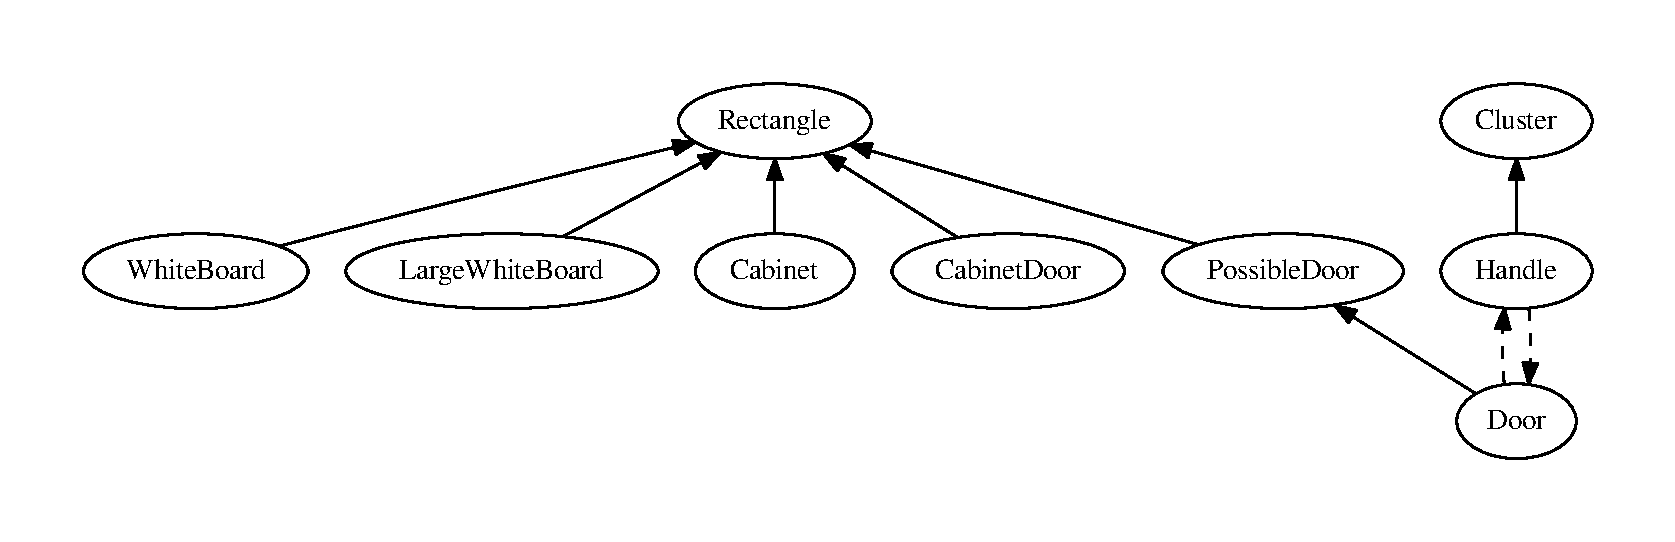
\includegraphics[width=\textwidth]{diagrammi/classifier}
  \caption{Grafo delle dipendenze}
  \label{fig:grafo-dipendenze}
\end{figure}

\begin{figure}[ht]
  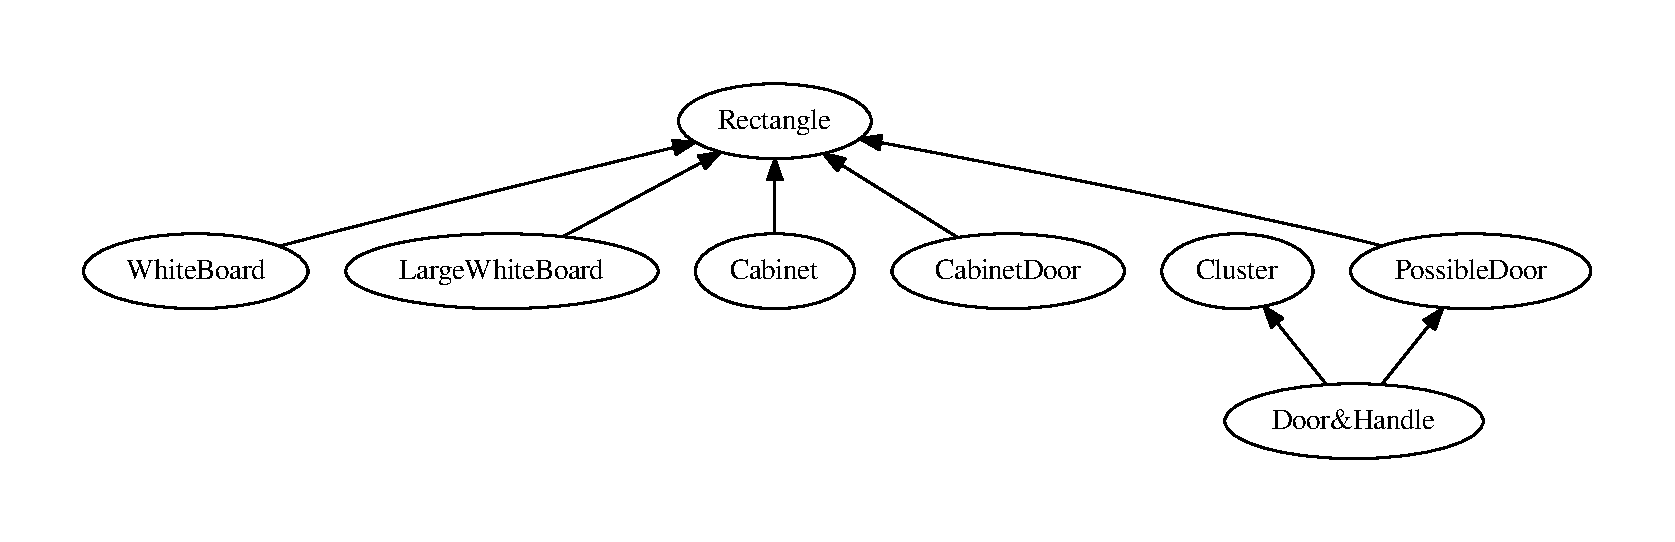
\includegraphics[width=\textwidth]{diagrammi/reasoning}
  \caption{Grafo di reasoning}
  \label{fig:grafo-reasoning}
\end{figure}


\end{document}
